% Author: Seongjin Lee 
% Hanyang University, Seoul, Korea 
% esos.hanyang.ac.kr 
% 2016-09-20
% note: some slides are adopted from  \url{www.cs.stevens.edu/~jschauma/631A/}
% https://github.com/resourceful/lecture_sysprog/

\documentclass[newPxFont,sthlmFooter,nooffset]{beamer}
\usepackage{kotex}
%\usetheme{sthlm}
\usepackage{../beamer_template/beamerthemesthlm}
\hypersetup{pdfauthor={Seongjin Lee (insight@hanyang.ac.kr)},
            pdfsubject={Lecture Note: System Programming},
            pdfkeywords={Lecture Note, System Programming, class, undergraduate},
            pdfmoddate={D: \pdfdate},
            pdfcreator={Seongjin Lee}}

%\setbeamertemplate{footline}[text line]{%
%    \parbox{\linewidth}{\vspace*{-8pt} \insertsectionhead  \hfill\insertshortauthor\hfill\insertpagenumber}}
%\setbeamertemplate{navigation symbols}{}




\title{System Programming}
\subtitle{Week 7: Process Relationships}
\author[SJL]{Seongjin Lee}
\institute{\href{mailto:insight@hanyang.ac.kr}{insight@hanyang.ac.kr}\\\url{http://esos.hanyang.ac.kr}\\Esos Lab. Hanyang University}
\date{2016-10-19} 

\begin{document}



\frame[plain]{\titlepage} 

\frame{\frametitle{Table of contents}\tableofcontents} 


%---------------------------------------------------------



\begin{frame}[t]
  \frametitle{introduction}
This chapter covers following items
  \begin{itemize}
  \item Terminal Logins
  \item 
  \item 
  \item 
  \end{itemize}

\end{frame}





\begin{frame}[t]
  \frametitle{Terminal}
  \begin{figure}[h]
    \centering
    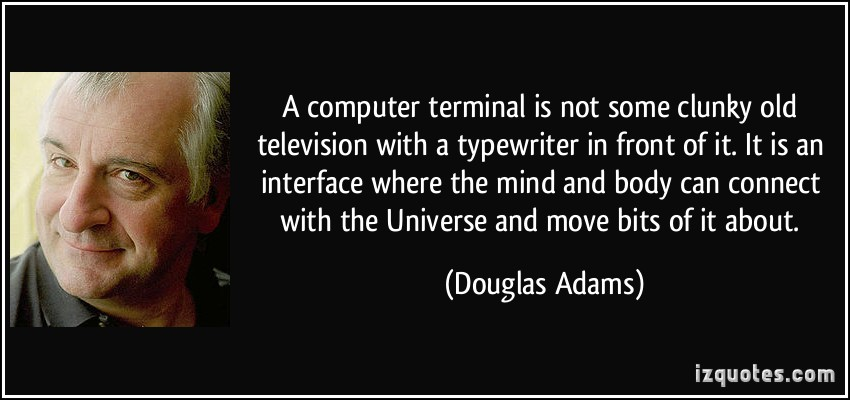
\includegraphics[width=0.8\linewidth]{figure/quote-a-computer-terminal-is-not-some-clunky-old-television-with-a-typewriter-in-front-of-it-it-is-an-douglas-adams-296711.jpg}
    \caption{Douglas Noel Adams was an English author, scriptwriter, essayist, humorist, satirist and dramatist, best known as the author of The Hitchhiker's Guide to the Galaxy'' 1978}
  \end{figure}
\end{frame}


\begin{frame}[fragile,t]
  \frametitle{Terminal Logins}
In early \textsc{Unix} systems
\begin{itemize}
\item <1-> Users logged in using dumb terminals that were connected to the host with hard-wired connections
\item <2-> The terminals were either local or remote
\item <3-> Users login through a terminal device driver in the kernel
\item <4-> A host had a fixed number of terminal devices

\item [ ] <5-> type \texttt{who} in the shell
\begin{verbatim}
James    console  Oct 12 15:36
James    ttys000  Oct 13 22:02
James    ttys001  Oct 13 22:08
\end{verbatim}
\end{itemize}
\end{frame}


\begin{frame}[t]
  \frametitle{BSD Terminal Logins}

Mac OS X and Linux login procedure follows essentially the same steps as the BSD 

The system administrator creates \texttt{/etc/ttys}, \texttt{ttys(5)}, that has one line per terminal device

Each line specifies the name of the device and other parameters that are passed to the \texttt{getty(8)} program
\end{frame}



\begin{frame}[t]
  \frametitle{BSD Terminal Logins cont'd}
  \begin{columns}[t]
    \begin{column}{0.6\linewidth}
      \begin{enumerate}
      \item <1-> the kernel creates process ID 1, the \texttt{init} process
      \item <2-> the \texttt{init} process reads the file \texttt{/etc/ttys}
      \item <2-> creates empty environment
      \item <3-> \texttt{fork}s for every terminal device
      \item <4-> followed by \texttt{exec} of the program \texttt{getty}
      \item <4-> opens terminal device (fd 0, 1, 2)
      \item <4-> reads user name
      \item <4-> initial environment set
      \item <5-> followed by \texttt{exec} of the program \texttt{login}
      \end{enumerate}
    \end{column}
    \begin{column}{0.4\linewidth}
      \begin{figure}[h]\vspace{-3em}
        \centering
        \begin{tikzpicture}
          \uncover<1-> { \node {\textit{process ID 1}}; } 
          \uncover<2->
          { \node [rectangle, minimum height=1cm, minimum width=2cm,
            draw] at (0,-1) {\texttt{init}}; } 
          \uncover<3-> { \draw
            [-Stealth, dashed] (-0.5,-1.5) -- (-1, -2); } 
          \uncover<3->
          { \draw [-Stealth, dashed] (0,-1.5) -- (0, -2.5); }
          \uncover<3-> { \draw [-Stealth, dashed] (0.5,-1.5) -- (1,
            -2) node [anchor=east] {\texttt{fork}}; } 
          \uncover<3-> {
            \draw
            [decorate,decoration={brace,amplitude=3pt},xshift=1.3cm,yshift=0pt]
            (0, -1.5) -- (0,-2.5) ; } 
          \uncover<3-> { \node [text
            width=2.5cm] at (2.8,-2) { \texttt{fork}s once per
              terminal }; }

          \uncover<3-> { \node [rectangle, minimum height=1cm, minimum
            width=2cm, draw] at (0,-3) {\texttt{init}}; }

          \uncover<4-> { \draw
            [decorate,decoration={brace,amplitude=3pt},xshift=1.3cm,yshift=0pt]
            (0, -3.5) -- (0,-4.5) ; } 
          \uncover<4-> { \node [text
            width=2.5cm] at (2.8,-4) { each child \texttt{exec}s
              \texttt{getty} }; } 
          \uncover<4-> { \draw [-Stealth]
            (0,-3.5) -- (0, -4.5) node [anchor= west,yshift=0.5cm]
            {\texttt{exec}}; }

          \uncover<4-> { \node [rectangle, minimum height=1cm, minimum
            width=2cm, draw] at (0,-5) {\texttt{getty}}; }

          \uncover<5-> { \draw [-Stealth]
            (0,-5.5) -- (0, -6.5) node [anchor= west,yshift=0.5cm]
            {\texttt{exec}}; }

          \uncover<5-> { \node [rectangle, minimum height=1cm, minimum
            width=2cm, draw] at (0,-7) {\texttt{login}}; }

        \end{tikzpicture}
      \end{figure}
    \end{column}

  \end{columns}

\end{frame}

\begin{frame}[t]
  \frametitle{BSD Terminal Logins}
  \begin{table}[h]
    \centering
    \begin{tabular}{m{6em}  *{3} {p{6em  }} }
      \texttt{init(8)} & PID 1 & PPID 0 & EUID 0  \\ 
      \multicolumn{4}{l}{\footnotesize reads \texttt{/etc/ttys}} \pause \\
      \texttt{getty(8)} & PID N & PPID 0 & EUID 0 \pause \\ 
      \multicolumn{4}{l}{\footnotesize opens terminal} \\
      \multicolumn{4}{l}{\footnotesize prints ``\texttt{login:}''}  \\
      \multicolumn{4}{l}{\footnotesize read username } \pause \\
      \texttt{login(1)} & PID N & PPID 0 & EUID 0 \\ 
      \multicolumn{4}{l}{\footnotesize \texttt{getpass(3)}, encrypt, compare with \texttt{getpwnam(3)}} \\
      \multicolumn{4}{l}{\footnotesize register login in system database} \\
      \multicolumn{4}{l}{\footnotesize read/display vaious files} \\
      \multicolumn{4}{l}{\footnotesize \texttt{initgroups(3)/setgid(2)}, initialize environment} \\
      \multicolumn{4}{l}{\footnotesize \texttt{chdir(2)} to home directory} \\
      \multicolumn{4}{l}{\footnotesize \texttt{chown(2)} terminal device} \\
      \multicolumn{4}{l}{\footnotesize \texttt{setuid(2)} to user's uid, \texttt{exec(3) shell}} \pause \\
      \texttt{\$SHELL} & PID N & PPID 0 & EUID U \pause \\ 
      \texttt{ls(1)} & PID M & PPID N & EUID U \pause \\ 
    \end{tabular}
  \end{table}
\end{frame}



%---------------------------------------------------------
\section{Last Words}

\begin{frame}[t]
  \frametitle{Last Words}
\begin{itemize}
\item 
\item 
\item 
\item 
\item 
\item 
\end{itemize}
\end{frame}

\end{document}
